% $Header$

\documentclass[
	xcolor=dvipsnames,
	hideallsubsections
]{beamer} %xcolor=dvipsnames
%\documentclass[xcolor=dvipsnames, handout]{beamer} %xcolor=dvipsnames

\usepackage{pgfpages}

\mode<presentation>
{
	\usetheme{PaloAlto}
	\usecolortheme[named=TealBlue]{structure}
%	\usecolortheme[named=Dandelion]{structure}
	
	\setbeamercovered{transparent}
	% or whatever (possibly just delete it)
%	\setbeameroption{show notes} % un-comment to see the notes
%	\setbeameroption{show notes on second screen=right}
}


%%%%%%%%%%%%%%%%%%%%%%%%%%%%%%%%%%%%%%%%%%%%%%%%%%%%%%%%%%%%%%%%%%%%%%%%%%%%%%%%%%%%%%%%%
% This LaTeX Beamer file is based on the solution template for:

% - Giving a talk on some subject.
% - The talk is between 15min and 45min long.
% - Style is ornate.

% Copyright 2004 by Till Tantau <tantau@users.sourceforge.net>.
%
% In principle, this file can be redistributed and/or modified under
% the terms of the GNU Public License, version 2.
%
% However, this file is supposed to be a template to be modified
% for your own needs. For this reason, if you use this file as a
% template and not specifically distribute it as part of a another
% package/program, I grant the extra permission to freely copy and
% modify this file as you see fit and even to delete this copyright
% notice. 
%%%%%%%%%%%%%%%%%%%%%%%%%%%%%%%%%%%%%%%%%%%%%%%%%%%%%%%%%%%%%%%%%%%%%%%%%%%%%%%%%%%%%%%%%

% Thank you so much Till :-)


\usepackage[ngerman]{babel}
% or whatever

\usepackage[latin1]{inputenc}
% or whatever

\usepackage{times}
\usepackage[T1]{fontenc}
 
%%%%%%%%%%%%%%%%%%%%%%%%%%%%%%%%%%%%%%%%%
% Arsclassica Article
% Structure Specification File
%
% This file has been downloaded from:
% http://www.LaTeXTemplates.com
%
% Original author:
% Lorenzo Pantieri (http://www.lorenzopantieri.net) with extensive modifications by:
% Vel (vel@latextemplates.com)
%
% License:
% CC BY-NC-SA 3.0 (http://creativecommons.org/licenses/by-nc-sa/3.0/)
%
%%%%%%%%%%%%%%%%%%%%%%%%%%%%%%%%%%%%%%%%%

%----------------------------------------------------------------------------------------
%	REQUIRED PACKAGES
%----------------------------------------------------------------------------------------

\usepackage[usenames,dvipsnames]{color} % Required for specifying custom colors and referring to colors by name

\usepackage[
nochapters, % Turn off chapters since this is an article        
beramono, % Use the Bera Mono font for monospaced text (\texttt)
%eulermath,% Use the Euler font for mathematics
eulerchapternumbers,
pdfspacing, % Makes use of pdftex’ letter spacing capabilities via the microtype package
dottedtoc % Dotted lines leading to the page numbers in the table of contents
]{classicthesis} % The layout is based on the Classic Thesis style

%\usepackage{arsclassica} % Modifies the Classic Thesis package

\usepackage[T1]{fontenc} % Use 8-bit encoding that has 256 glyphs

\usepackage[utf8]{inputenc} % Required for including letters with accents

\usepackage{graphicx} % Required for including images
\graphicspath{{Figures/}} % Set the default folder for images

\usepackage{enumitem} % Required for manipulating the whitespace between and within lists

\usepackage{lipsum} % Used for inserting dummy 'Lorem ipsum' text into the template

\usepackage{amsmath,amssymb,amsthm} % For including math equations, theorems, symbols, etc

\usepackage{varioref} % More descriptive referencing

\usepackage{url}

\usepackage{hyperref}

\usepackage{gensymb}	%for the \degree command

\usepackage[ngerman, english]{babel}

\usepackage[square,
authoryear,
%numbers,
longnamesfirst
]{natbib}

\usepackage{enumitem}

\usepackage{authblk}

\usepackage{relsize, etoolbox, lmodern}% http://ctan.org/pkg/{relsize,etoolbox}

\AtBeginEnvironment{quote}{\smaller\fontfamily{lmss}\selectfont}% Step font down one size relative to current font.
% see http://tex.stackexchange.com/questions/25249/how-do-i-use-a-particular-font-for-a-small-section-of-text-in-my-document for fontfamilies

\usepackage{chngcntr}

% to have a separation in the text with extra space between paragraphs and no indendation following
\newcommand*{\skippingparagraph}{\par\vspace{1.0\baselineskip}\noindent}

%----------------------------------------------------------------------------------------
%	HYPERLINKS
%---------------------------------------------------------------------------------------
\definecolor{mediumviolet-red}{rgb}{0.78, 0.08, 0.52}
\hypersetup{
%	draft, % Uncomment to remove all links (useful for printing in black and white)
	colorlinks=true, breaklinks=true, bookmarks=true,bookmarksnumbered,
	urlcolor=webbrown, linkcolor=mediumviolet-red, citecolor=webgreen, % Link colors
	pdftitle={}, % PDF title
	pdfauthor={\textcopyright}, % PDF Author
	pdfsubject={}, % PDF Subject
	pdfkeywords={}, % PDF Keywords
	pdfcreator={pdfLaTeX}, % PDF Creator
	pdfproducer={LaTeX with hyperref and ClassicThesis} % PDF producer
}

%----------------------------------------------------------------------------------------
%	TODONOTES
%---------------------------------------------------------------------------------------

\usepackage[colorinlistoftodos]{todonotes}

\newcommand{\todoInfo}[1]{\todo[color=blue!25]{INFO: #1}}
\newcommand{\todoCite}[1]{\todo[color=green!40]{INFO: #1}}


%----------------------------------------------------------------------------------------
%	CODESNIPPETS
%---------------------------------------------------------------------------------------

%%%%%%%%%%%%%%%%%%%%%%%%%%%%%%%%%%%%%%%%%
% Code Snippet
% LaTeX Template
% Version 1.0 (14/2/13)
%
% This template has been downloaded from:
% http://www.LaTeXTemplates.com
%
% Original author:
% Velimir Gayevskiy (vel@latextemplates.com)
%
% License:
% CC BY-NC-SA 3.0 (http://creativecommons.org/licenses/by-nc-sa/3.0/)
%
%%%%%%%%%%%%%%%%%%%%%%%%%%%%%%%%%%%%%%%%%
\usepackage{listings} % Required for inserting code snippets

\definecolor{DarkGreen}{rgb}{0.0,0.4,0.0} % Comment color
\definecolor{highlight}{RGB}{255,251,204} % Code highlight color
\definecolor{DogwoodRose}{rgb}{0.84, 0.09, 0.41}
\definecolor{lemonchiffon}{rgb}{1.0, 0.98, 0.8}
\definecolor{lightgoldenrodyellow}{rgb}{0.98, 0.98, 0.82}
\definecolor{oldlace}{rgb}{0.99, 0.96, 0.9}
\definecolor{oldlavender}{rgb}{0.47, 0.41, 0.47}
\definecolor{pakistangreen}{rgb}{0.0, 0.4, 0.0}
\definecolor{ao}{rgb}{0.0, 0.0, 1.0}
\definecolor{britishracinggreen}{rgb}{0.0, 0.26, 0.15}
\definecolor{coquelicot}{rgb}{1.0, 0.22, 0.0}
\definecolor{cordovan}{rgb}{0.54, 0.25, 0.27}
\definecolor{darkcandyapplered}{rgb}{0.64, 0.0, 0.0}
\definecolor{mediumchampagne}{rgb}{0.95, 0.9, 0.67}

\lstdefinestyle{Style1}{ % Define a style for your code snippet, multiple definitions can be made if, for example, you wish to insert multiple code snippets using different programming languages into one document
	language=JavaScript, % Detects keywords, comments, strings, functions, etc for the language specified
	backgroundcolor=\color{oldlace}, % Set the background color for the snippet - useful for highlighting
	basicstyle=\smaller\smaller\ttfamily, % The default font size and style of the code
	breakatwhitespace=true, % If true, only allows line breaks at white space
	breaklines=true, % Automatic line breaking (prevents code from protruding outside the box)
	captionpos=b, % Sets the caption position: b for bottom; t for top
	commentstyle=\usefont{T1}{pcr}{m}{sl}\color{ao}, % {m}DarkGreen Style of comments within the code - dark green courier font
	deletekeywords={}, % If you want to delete any keywords from the current language separate them by commas
	%escapeinside={\%}, % This allows you to escape to LaTeX using the character in the bracket
	firstnumber=1, % Line numbers begin at line 1
	frame=single, % Frame around the code box, value can be: none, leftline, topline, bottomline, lines, single, shadowbox
	frameround=tttt, % Rounds the corners of the frame for the top left, top right, bottom left and bottom right positions
	keywordstyle=\color{darkcandyapplered}\textbf, % Functions are bold and blue
	morekeywords={}, % Add any functions no included by default here separated by commas
	numbers=left, % Location of line numbers, can take the values of: none, left, right
	numbersep=10pt, % Distance of line numbers from the code box
	numberstyle=\tiny\color{Gray}, % Style used for line numbers
	rulecolor=\color{black}, % Frame border color
	showstringspaces=false, % Don't put marks in string spaces
	showtabs=false, % Display tabs in the code as lines
	stepnumber=5, % The step distance between line numbers, i.e. how often will lines be numbered
	stringstyle=\color{Purple}, % Strings are purple
	tabsize=2, % Number of spaces per tab in the code
}

\definecolor{darkgray}{rgb}{.4,.4,.4}
\definecolor{purple}{rgb}{0.65, 0.12, 0.82}


%define Javascript language
\lstdefinelanguage{JavaScript}{
	keywords={typeof, new, true, false, catch, try, finally, function, return, null, then, catch, switch, var, if, in, while, do, else, case, break, yield, async, await},
	keywordstyle=\color{blue}\bfseries,
	ndkeywords={class, export, boolean, throw, implements, import, this},
	ndkeywordstyle=\color{darkgray}\bfseries,
	identifierstyle=\color{black},
	sensitive=false,
	comment=[l]{//},
	morecomment=[s]{/*}{*/},
	commentstyle=\color{purple}\ttfamily,
	stringstyle=\color{red}\ttfamily,
	morestring=[b]',
	morestring=[b]"
}

\lstset{
	language=JavaScript,
	extendedchars=true,
	basicstyle=\footnotesize\ttfamily,
	showstringspaces=false,
	showspaces=false,
	numbers=left,
	numberstyle=\footnotesize,
	numbersep=9pt,
	tabsize=2,
	breaklines=true,
	showtabs=false,
	captionpos=b
}

% Create a command to cleanly insert a snippet with the style above anywhere in the document
\newcommand{\insertcode}[2]{\begin{itemize}\item[]\lstinputlisting[{caption={#2}},label=#1,style=Style1]{#1}\end{itemize}} % The first argument is the script location/filename and the second is a caption for the listing
 % Include the structure.tex file which specified the document structure and layout


% Or whatever. Note that the encoding and the font should match. If T1
% does not look nice, try deleting the line with the fontenc.

\title[Notlandefelder aus H�hendaten] % (optional, use only with long paper titles)
{Erkennung von Notlandefeldern aus H�hendaten: \\
	Parallele Implementierung der Durchmusterung mit \texttt{pThreads}}

\author[] % (optional, use only with lots of authors)
{Felix~Eckstein, Dr. Bj�rn Wittich}
% - Use the \inst{?} command only if the authors have different
%   affiliation.

%\institute[FernUni Hagen] % (optional, but mostly needed)
%{
%}
  
% - Use the \inst command only if there are several affiliations.
% - Keep it simple, no one is interested in your street address.

\date[] % (optional)
{``1597 -- Fachpraktikum Parallele Programmierung''\\
	im Sommersemester 2017 an der FernUniversit�t Hagen\\
23. September 2017}

\subject{Talks}
% This is only inserted into the PDF information catalog. Can be left
% out. 



% If you have a file called "university-logo-filename.xxx", where xxx
% is a graphic format that can be processed by latex or pdflatex,
% resp., then you can add a logo as follows:

% \pgfdeclareimage[height=1cm]{university-logo}{images/HannoverJs.png}
  \pgfdeclareimage[height=1cm]{university-logo}{images/UniHagen.png}
 \logo{\pgfuseimage{university-logo}}



% Delete this, if you do not want the table of contents to pop up at
% the beginning of each subsection:
\AtBeginSection[]
{
  \begin{frame}<beamer>{Outline}
%    \tableofcontents[currentsection]%,currentsubsection]
    \tableofcontents[sections=\thesection]
  \end{frame}
}

\begin{document}

\begin{frame}
  \titlepage
	\note{
		\begin{itemize}
			\item In den \textbackslash note Abschnitt kommen Vortragsnotizen
			\item \ldots
		\end{itemize}
			
	Kein Vortrag ohne Katzenfotos!
	}
\end{frame}



\begin{frame}{Outline}
  	\tableofcontents[hideallsubsections]
	\note{
		\begin{itemize}
			\item In den \textbackslash note Abschnitt kommen Vortragsnotizen
			\item \ldots
		\end{itemize}
			
	Kein Vortrag ohne Katzenfotos!
	}
\end{frame}


% Since this a solution template for a generic talk, very little can
% be said about how it should be structured. However, the talk length
% of between 15min and 45min and the theme suggest that you stick to
% the following rules:  

% - Exactly two or three sections (other than the summary).
% - At *most* three subsections per section.
% - Talk about 30s to 2min per frame. So there should be between about
%   15 and 30 frames, all told.

\setcounter{framenumber}{\value{framenumber}-1}	%no idea why it otherwise skips one page
\section{Aufgabenstellung}

\begin{frame}{Funktionsaufrufe in Single-Threaded-Umgebungen}{``Synchrone Programmierung''}
	
	\begin{columns}
		\column{0.5\textwidth}
		\begin{itemize}[<+->]
			\item Synchrone Funktionen
			\begin{itemize}[<.->]
				\item werden aufgerufen
				\item berechnen ihr Ergebnis
				\item geben das Resultat zur�ck
			\end{itemize}
			\item Funktionsaufrufe k�nnen die Ausf�hrung blockieren
			\item Das Warten auf externe Ereignisse f�hrt zu Ineffizienz
			\item Es ist keine Neben- l�ufigkeit m�glich
		\end{itemize}
		\column{0.5\textwidth}
			\begin{figure}
				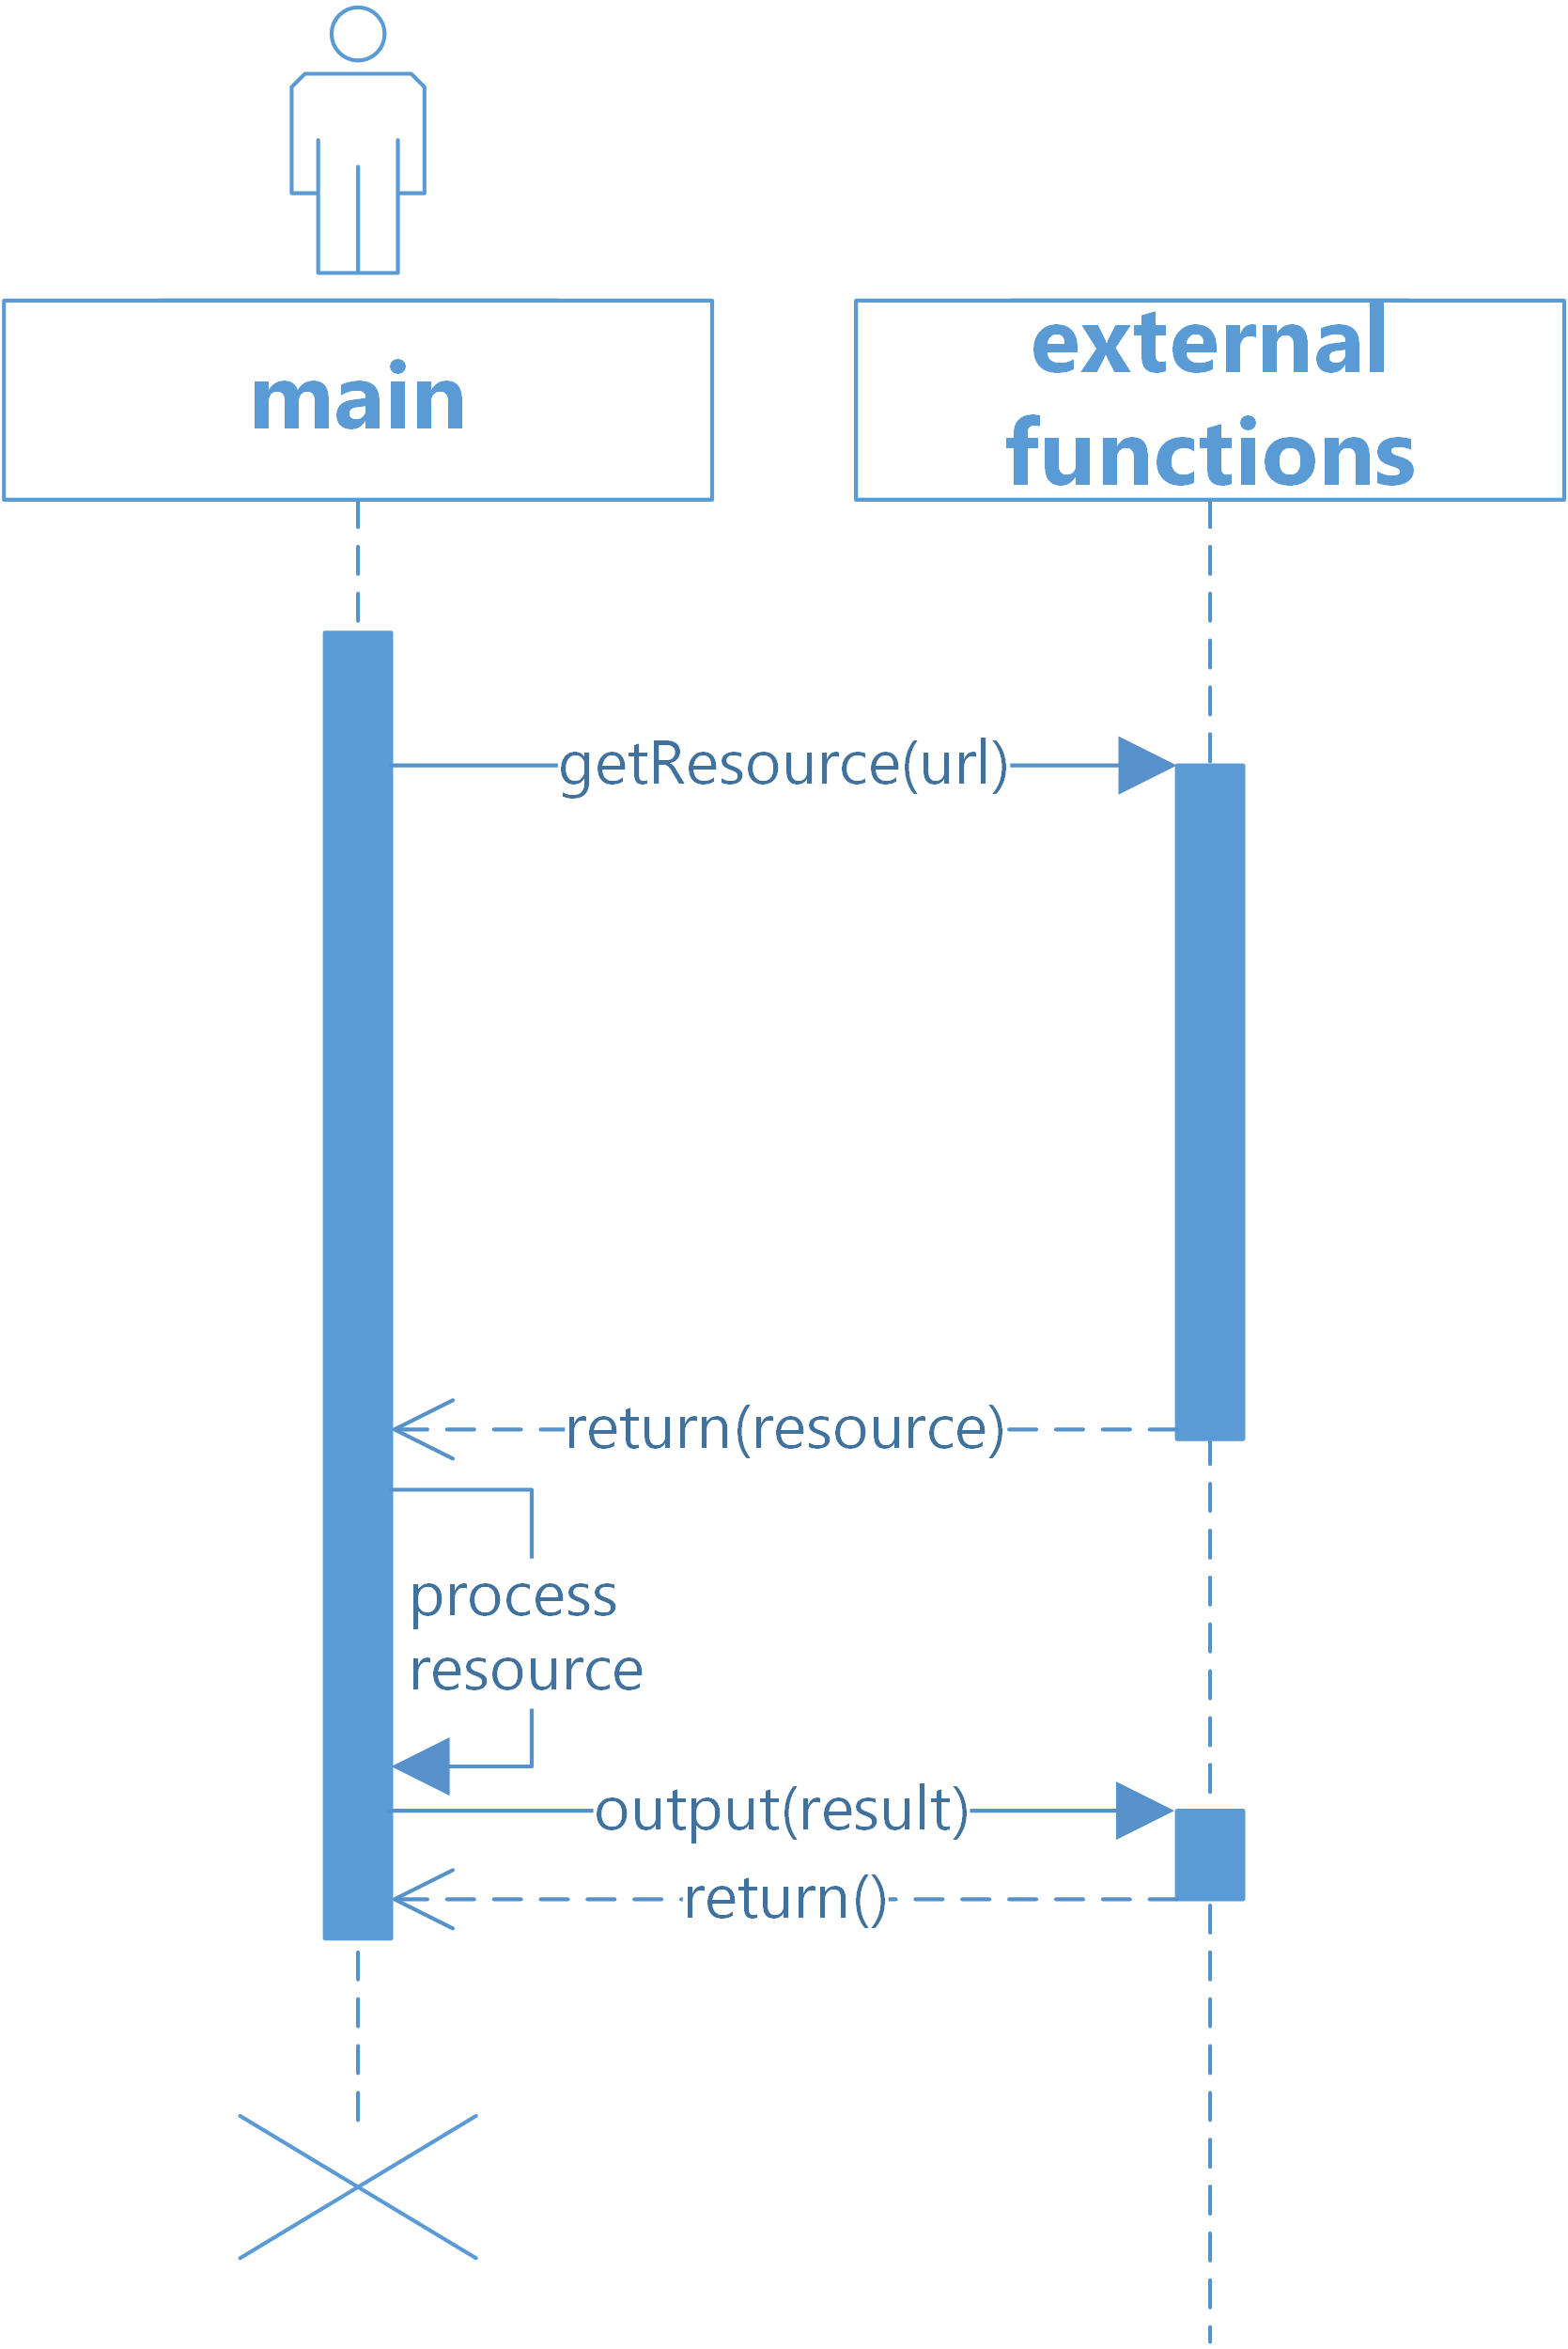
\includegraphics[height=.8\textheight]{images/syncFlow.png}
			\end{figure}
	\end{columns}

	\note{
		\begin{itemize}
			\item Das Hauptprogramm kann nicht weiterarbeiten
			\item Nebenl�ufigkeit ist nicht m�glich
			
			\skippingparagraph
			
			\skippingparagraph
			
			\item Was l�sst sich daran besser machen?
		\end{itemize}
	}

\end{frame}

	\begin{frame}{Asynchrone Programmierung}
		
	\begin{itemize}[<+->]
		\item<1-> Asynchrone Funktionen verhalten sich anders:	
		\begin{itemize}[<+->]
			\item<+-> Async Funktionen werden \alert{jetzt} aufgerufen, \ldots
			\item<+-> \ldots kehren direkt zur�ck\ldots
			\item<+-> \ldots und berechnen ihr Ergebnis
			\item<+-> Diese Ergebnis wird \alert{sp�ter} �bergeben
		\end{itemize}
		\item<+-> Der aufrufende Code erh�lt die Kontrolle direkt zur�ck
		\item<+-> Das Hauptprogramm kann sinnvolle Dinge tun, w�hrend die async Funktion noch ihr Ergebnis ermittelt
		\item<+-> Dadurch gibt es \alert{Nebenl�ufigkeit} auch in single-threaded Umgebungen
	\end{itemize}

	\note{
		Erkl�re hier, dass die asynchronen Funktionen eben \alert{doch in einem anderen Thread} ablaufen k�nnen.

		Eventuell sogar noch die Grafik Zeigen: 
		
		\begin{figure}
			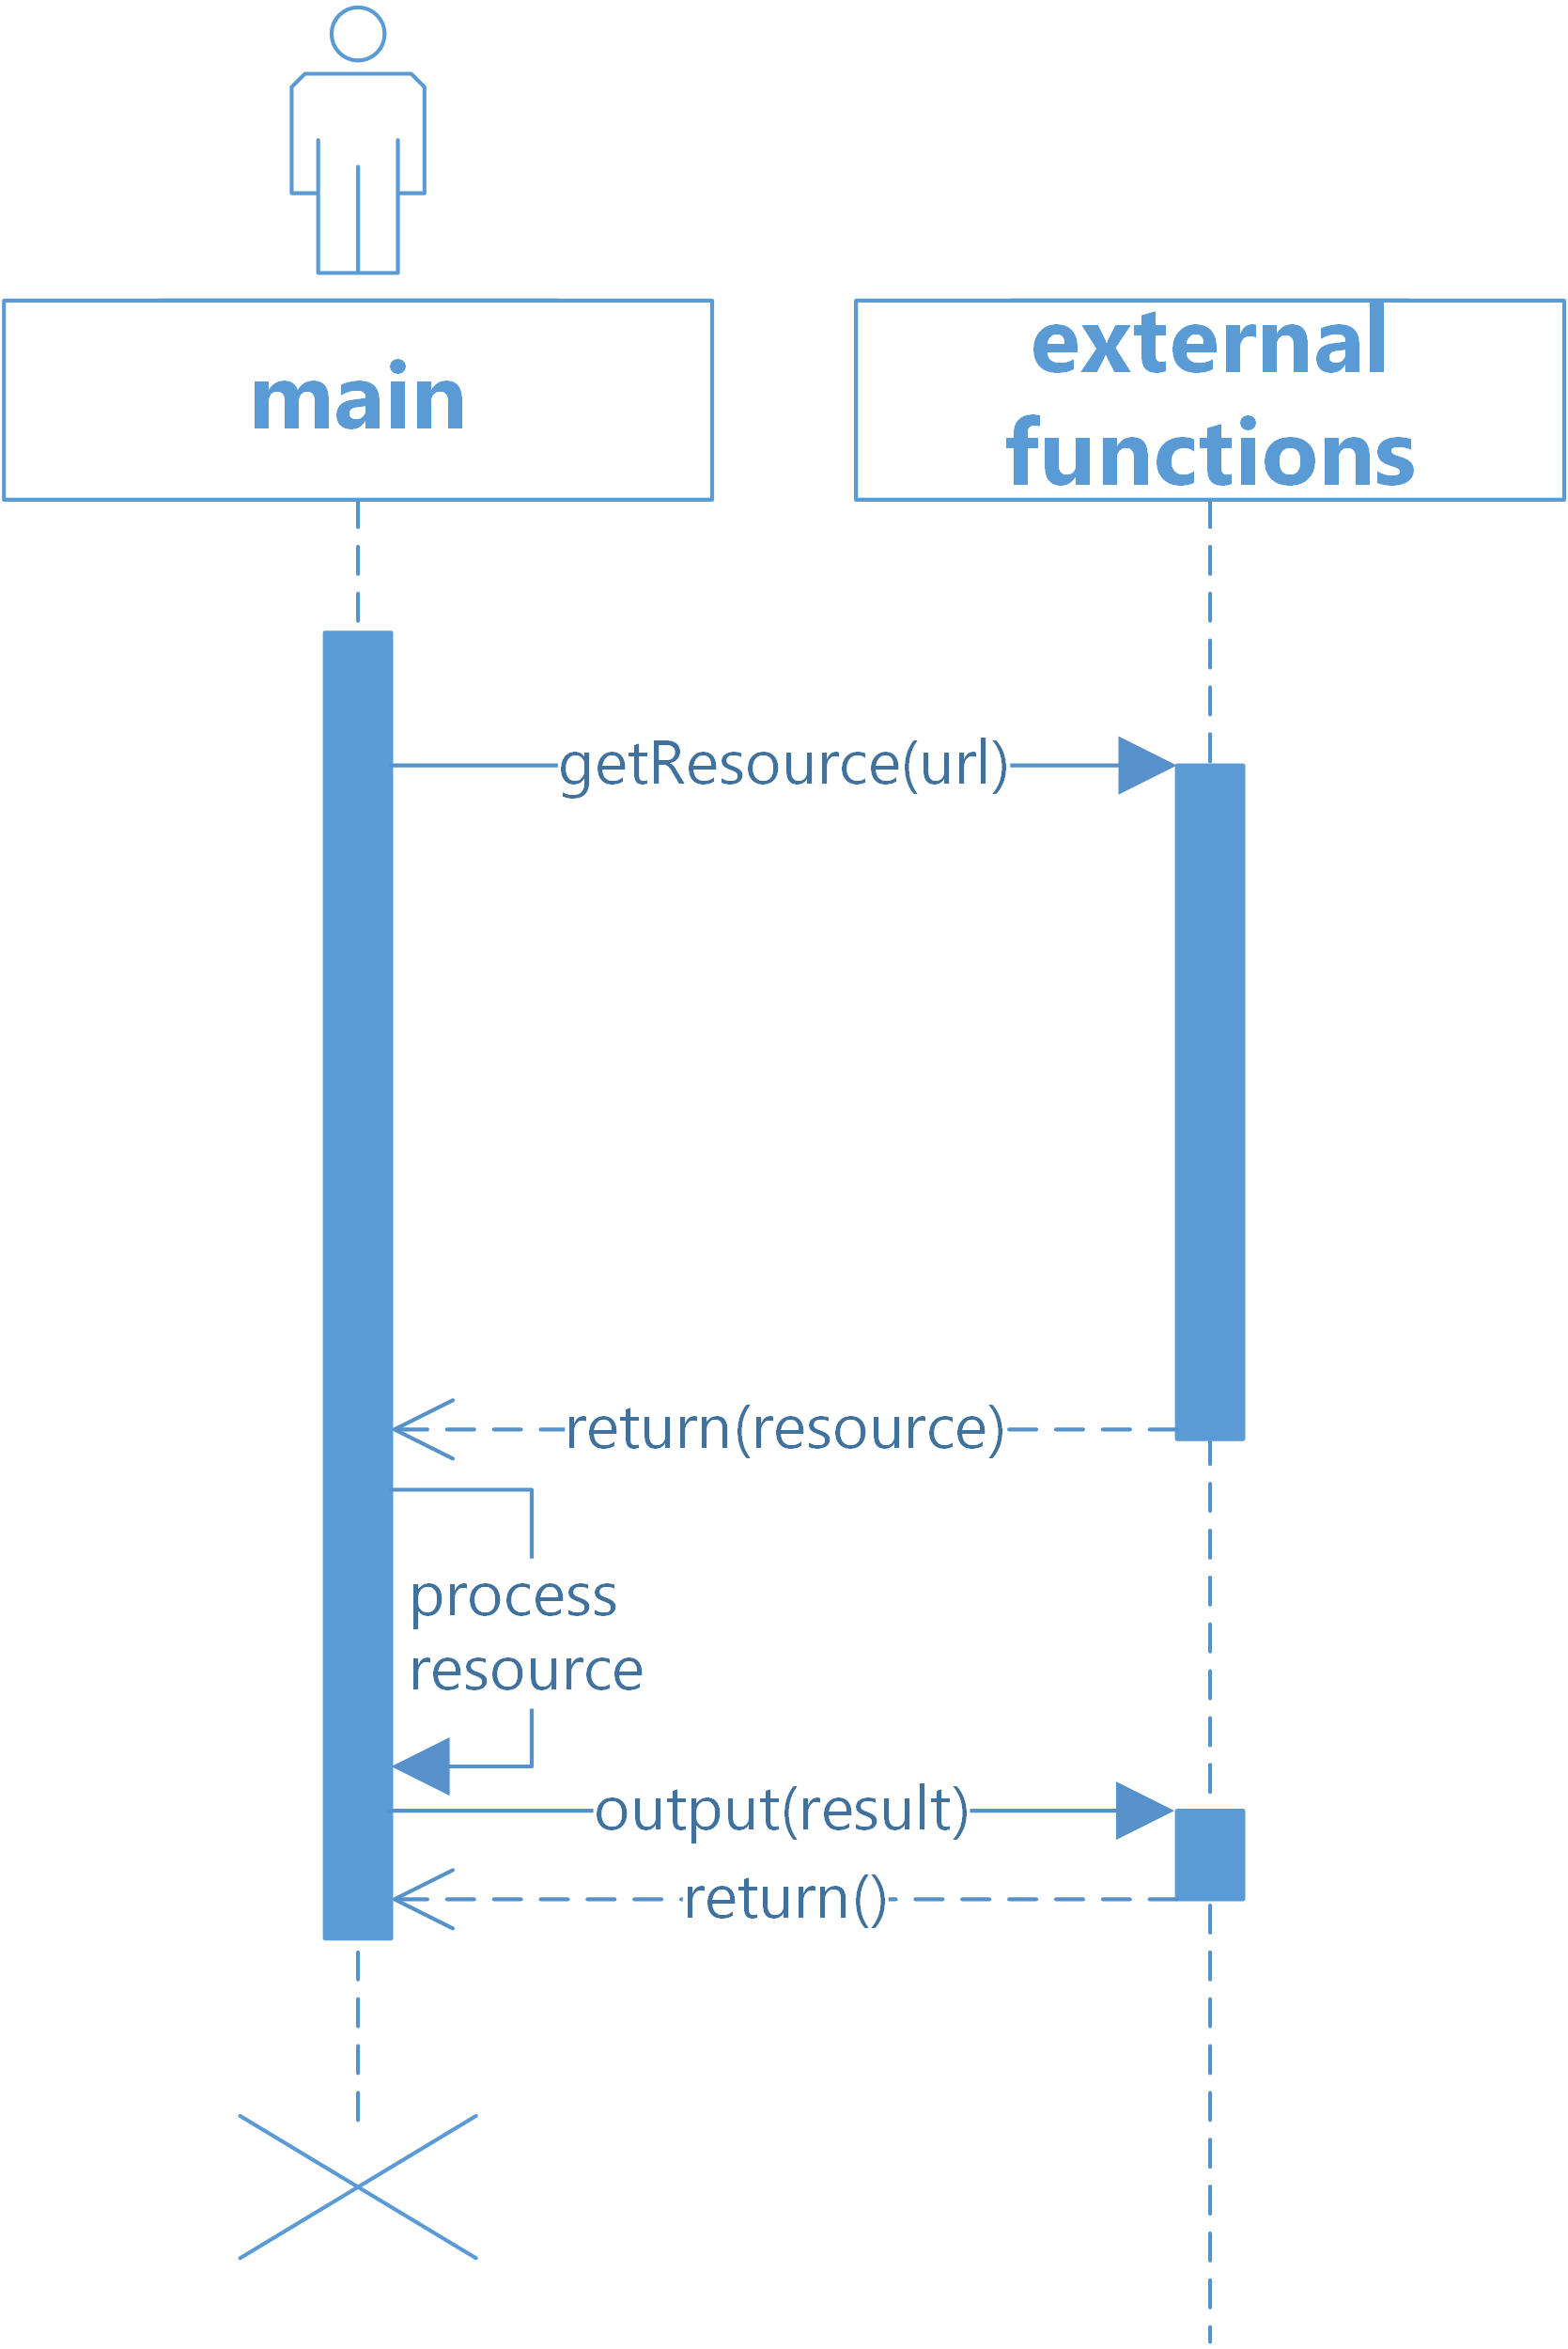
\includegraphics[height=.5\textheight]{images/syncFlow.png}
			\caption{Asnychronous Functions are executed outside the JavaScript-Single-Thread}
		\end{figure}
		
	}
	\end{frame}
	
\section{Architektur}
\subsection{�berblick}
\subsection{Grobk�rnige Parallelit�t}
\subsection{Feingranulare Parallelit�t}

\section{Komponente "`searchEngine"'}

\subsection{Datenformate und Verarbeitung}
\subsubsection{GeoTIFF}
\subsubsection{Speicherformat: GeoJSON}
\subsection{GeoTIFFHandler}
\subsubsection{Datenextraktion}
\subsubsection{Koordinatensysteme}
\subsubsection{Das \texttt{GeoTIFFHandler}-Objekt}


\section{Komponente "'Durchmusterung"'}
\subsection{Durchmusterung der Geotiff Daten und Auffinden der Landebahnen}

\subsection{Interface der Library}

\subsection{Logischer Ablauf innerhalb der Landebahn-Erkennung}

\subsection{Initialisierung}

\subsection{Parallelverarbeitung mittels p\_threads zum Finden der Landebahnen}

\subsection{Detaillierte Beschreibung des Suchalgorithmus}

\subsection{Klassen und Objekte}

\subsection{Verwendete Datenstrukturen}

\subsubsection{Einfluss der Datenstrukturen auf die Performanz}

\subsection{Bestimmung des Speedups in Abh�ngigkeit des Parallelisierungsgrades}

\subsubsection{Erl�uterung des Messverfahren}

\subsubsection{Messergebnisse}

\subsubsection{Diskussion der Messergebnisse}

\subsection{Analyse mittels Profiler}

\subsection{Einfluss von Compiler Direktiven (speziell Optimizer)}

\section{Komponente "`databaseManager"'}

\subsection{Datenbankauswahl}

	\begin{frame}{Ein GeoJSON Objekt zur Ablage in die Datenbank}{}
			
		\smaller\lstinputlisting[style=JSStyle, linebackgroundcolor={%
			\btLstHL<2|handout:0>{18}%
			\btLstHL<3|handout:0>{19,20}% 
		}]{snippets/databaseObject.js}
		
	\end{frame}
	


	\subsection{Express-Server App}
	
	\subsection{Postprocessing - Merge}
	
	\section{Komponente "'landingClient"'}
	
	\begin{frame}{Benutzeroberfl�che}
		\begin{figure}[ht]
			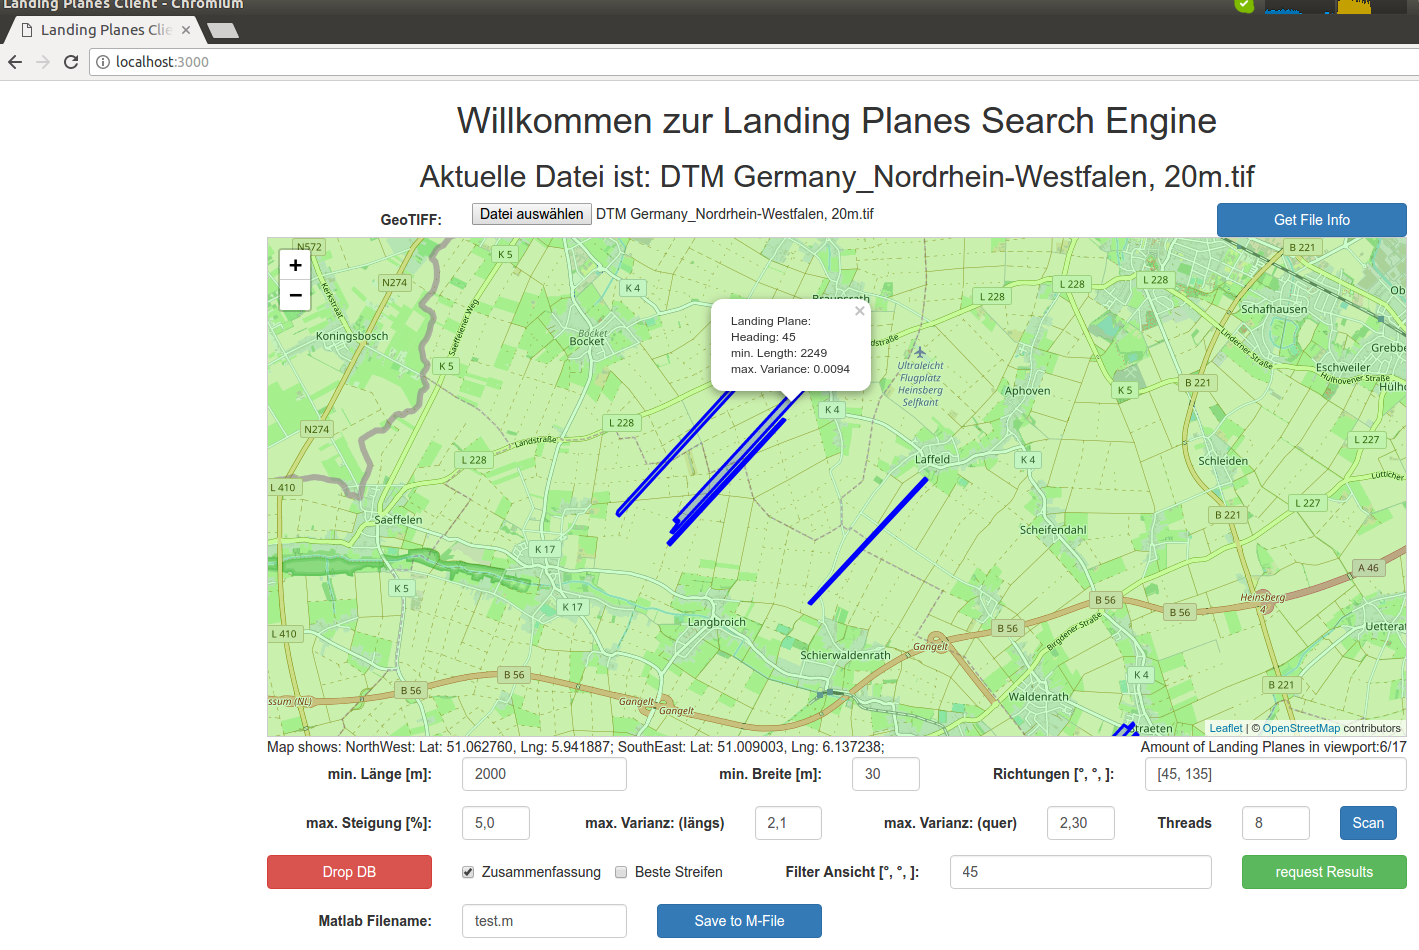
\includegraphics[width=\textwidth]{../Bericht/drawings/LandingClient_Screen1.png}
			\caption{Beispiel Screenshot aus der Weboberfl�che zur Bedienung des Systems}
		\end{figure}
	\end{frame}
	
	\subsection{�berblick}
	
	\subsection{Features und Bedienung}
	
	\section{Ausblick und weitere Ideen}
	
	\subsection{Parallele Bearbeitung mehrerer Kacheln per MPI}
	
	\subsection{Richtungskorrektur des GeoTIFF}
	
	\subsection{Push f�r Webclient}
	
	\subsection{Merge als nachgeschalteter Prozess aus dem Speicher}
	
	\subsection{Kollisionsabfrage mit Objekten aus OSM}
	
\end{document}


